% Section name and highlighted ToC
%\renewcommand{\sectiontitle}{Introduction}
%\section{\sectiontitle}
%\customToC{currentsection,hideothersubsections}{}

% Section name and highlighted ToC
%\renewcommand{\subsectiontitle}{What is machine learning?}
%\subsection{\subsectiontitle}


\begin{frame}{Overview}
  \tableofcontents
\end{frame}
%%%% Work summary 
\section{Last week queries}
\begin{frame}
  \frametitle{On the Error of Random Fourier Features}

  \begin{itemize}
    \item Authors: Danica J. Sutherland and Jeff Schneider
    \item Year 2015.
    \item Cited by 185. 
    \item See \cite{sutherland2015error}
  \end{itemize}

  Why is interesting
  \begin{itemize}
    \item Which of two embedding is interesting. 
    \item Error considerations.  
  \end{itemize}

\end{frame}

\begin{frame}
  \frametitle{Two embdedding based on Fourier tansform}
  
  One of the form: 
  \begin{equation}
    \tilde{z}(x) = \sqrt{\frac{2}{D}}
    [\sin(w_1^T x) \cos(w_1^T x) \ldots \sin(w_{D/2}^T x) \cos(w_{D/2}^T x)]^T, w_i \sim P
  \end{equation}
  and another of the form 
  \begin{equation}
    \breve{z}(x) = \sqrt{\frac{2}{D}}
    [\cos(w_1^T x + b_1) \ldots \cos(w_{D}^T x + b_D)]^T, w_i \sim P, b_i \sim Unif([0, 2\pi])
  \end{equation}

\end{frame}

\begin{frame}
  \frametitle{Kernel approximation}
  \begin{equation}
    \tilde{s}(x,y)
    = 
    \frac{1}{D/2} \sum_{i=1}^{D/2}
    \cos(w_i^T(x-y))
  \end{equation}

  \begin{equation}
    \breve{s}(x,y)
    = 
    \frac{1}{D} \sum_{i=1}^{D}
    \cos(w_i^T(x-y))
    +
    \cos(w_i^T(x+b) + 2b_i)
  \end{equation}
  

\end{frame}

\begin{frame}
  \frametitle{Models comparatives}
\begin{itemize}
  \item of the first 100 papers cit-
  ing Rahimi and Recht (2007) in a Google Scholar search,
  used either  $\tilde{z}$ or the equivalent formulation.
  \item The article show that $\tilde{z}$ is superior for Gaussian kernel. 
  Providing a complementary view of the quality of
these embeddings:
  \begin{itemize}
    \item Variance of each embedding $\tilde{s}$ for RBF uniformly lower variance.
    \item Uniform convergence bounds, tightening constants in the
    original $\tilde{z}$ (one worse).
    \item $L_2$ convergence of each approximation $\tilde{z}$ superior again.
    \item Finally empirically. 
  \end{itemize}
\end{itemize}
  

\end{frame}


\section{Article information}
\begin{frame}{Random Features for Kernel Approximation: A Survey on Algorithms, Theory, and Beyond}
  \begin{itemize}
    \item Fanghui Liu and Xiaolin Huang and Yudong Chen and Johan A. K. Suykens
    \item Year 2021
    \item Cited by 94!!!
  \end{itemize}
  \cite{liu2021random}
 
\end{frame}

\section{Theoretical Foundation of Random Features}

\begin{frame}
  \frametitle{Theoretical Foundation of Random Features}

  \begin{theorem}{Bochner’s Theorem}
    A continuous and shift-invariant function $k :\R^d  \times \R^d \longrightarrow \R$ 
is positive definite if and only
if it can be represented as
\begin{equation}
  k(x - x')
  = 
  \int_{\R^d} 
    \exp{i w^T (x - x')}
    \mu_k( d_w)
\end{equation}
where $\mu_k$ is a is a positive finite measure on the frequencies 
$w$. 
\end{theorem}
  
According to Bochner's theorem, the spectral distribution $\mu_k$
of a stationary kernel $k$ is the finite measure induced by a Fourier
transform.
\end{frame}


\begin{frame}

  By setting $k(0) = 1$, we may normalize $\mu_k$ to a
probability density $p$ (the Fourier transform associated with $k$),
hence

\begin{align}
  k(x - x')
  & =  
  \int_{\R^d} 
    \exp{i w^T (x - x')}
    \mu( d_w)
  \\ & =  
  E_{w \sim p }
  \left[
    exp{(i w^T x )}
    exp{(i w^T x')^*}, 
  \right]
\end{align}
The
  kernels used in practice are typically real-valued and thus the
  imaginary part can be discarded.

\end{frame}

\begin{frame}

\begin{equation}
  \varphi_p(x)
  = 
  \left[
    exp{(- i w_1^T x )},
    \ldots,
    exp{(-i w^T_s x)}
  \right]^T.
\end{equation}

\end{frame}

\begin{frame}
  \frametitle{ Two-layer network correspondence to random features approximation}

  \textbf{Given a two-layer network}

  \begin{equation*}
    f(x;\theta)
    = 
    \sqrt{\frac{2}{s}}
    \sum_{j = 1}^s 
    a_j \sigma(w_j^T x)
  \end{equation*}
  for some activation function $\sigma$ and $x \in \R^d$
  when $w \sim \mathcal{N}(0, I_d)$ and only the second layer are optimized this correspond to random features approximation 

  \begin{equation}
    k(x, x')
    = 
    E_{w \sim \mathcal{N}(0, I_d)}
    \left[
    \sigma{( w^T x )}
    \sigma{( w^T x')}, 
  \right]
  \end{equation}
  depends on the
  kernel type such that 
  \begin{equation}
    \varphi(x) := \sigma(Wx). 
  \end{equation}
  
\end{frame}

\begin{frame}
  \frametitle{Some examples:}

  \begin{itemize}
    \item Correspond to a standard RFF model for a Gaussian kernel: 
    \begin{equation}
      \sigma(x) = \left[ \cos(x) \sin(x)\right]
    \end{equation}
    \item First order arc-cosine kernel 
    termed as 
    \begin{equation}
      k(x, x')
      = 
      k(u)
      = 
      \frac{1}{\pi}(u (\pi - \arccos(u))+ \sqrt{1 -u^2})
    \end{equation}
    where 
    \begin{equation}
      u = \frac{\langle x, x' \rangle}{\|x\|\|x'\|}
    \end{equation}
    if $\sigma(x) = \max\{0,x\}$. 
  \end{itemize}
\end{frame}

\begin{frame}
  \frametitle{For fully connected deep neural network}

  Pregunta: 
  Una red neuronal de dos capas representa un kernel. 
  Ese kernel se puede aproximar a una red neuronales de una capa oculta. 
  LUEGO SE ESTARÍA TRANSFORMANDO LAS REDES NEURALES DE UNA CAPA A OTRA.

  Referencias que ver \cite{daniely2017deeper} and \cite{lee2018deep} and from the origin article references (12, 63,64,65,66,67 and 68).
\end{frame}


\begin{frame}
  \frametitle{Commonly used kernels in Random Features}

  Actually not interesting 

\end{frame}

\section{Taxonomy of random features based algorithms}
\begin{frame}
  \frametitle{Taxonomy of random features based algorithms}

  \begin{equation}
    \varphi(x)
    = 
    \left[
     a_1 \exp{(- i w_1^T x )},
      \ldots,
     a_s exp{(-i w^T_s x)}, 
    \right]^T
  \end{equation}

They can be grouped into two categories,
data-independent algorithms and data-dependent algorithms, based
on whether or not the selection of $w_i$ and $a_i$ is independent of the
training data

See figure 2 of the article. 

And \cite{NIPS2008_0efe3284} is improved by \cite{le2014fastfood}
\end{frame}

\section{Theoretical Analysis}
\begin{frame}
  \frametitle{Error approaches }


\begin{itemize}
  \item \textbf{Approximation}: how many random features are needed to
  ensure a high quality estimator in kernel approximation?
  \item \textbf{Generalization} how many random features are needed to
  incur no loss of empirical risk and expected risk in a learning
  estimator?

  \begin{itemize}
    \item See convergences on table 3 of \cite{liu2021random}. 
    \item Rates and required random features in table 4.
    \item Comparison of learning rates and required random features for expected risk with a Lipschitz continuous loss function. Table 5. 
  \end{itemize}

\end{itemize}
  

\end{frame}


\begin{frame}
  \frametitle{Other comparation and interesting fields}
\begin{itemize}
  \item Space and time complexities see table 2 page 8 of \cite{liu2021random}.
  \item Trends: High-dimensional Random Features in Over parameterized settings (page 21)
  \begin{itemize}
    \item Double descent in the
    test error curve (as we saw in DNN)
  \end{itemize}
\end{itemize}
  

\end{frame}

\begin{frame}
  \frametitle{Future}

  RFF in DNNs!!!
  See references Figure 1 \cite{liu2021random}.

\end{frame}

\begin{frame}
  \frametitle{Next week: Neural Network? }

  \begin{enumerate}
    \item \textbf{Nystroem Method vs Random Fourier Features: A Theoretical and Empirical Comparison, Advances in Neural Information Processing Systems 2012}
    
    \item \textbf{Random features for kernel approximation: A survey on algorithms, theory, and beyond}
    \item \textbf{Williams, C.K.I. and Seeger, M. “Using the Nystroem method to speed up kernel machines”, Advances in neural information processing systems 2001
    T. Yang, Y. Li, M. Mahdavi, R. Jin and Z. Zhou }
    \item Weighted Sums of Random Kitchen Sinks: Replacing minimization with randomization in learning.
    \item Randomness in neural networks: an overview
    \item Fast and scalable polynomial kernels via explicit feature maps
    \item \textbf{On the error of random Fourier features}
    \item A survey on large-scale machine learning
    \item Sharp analysis of low-rank kernel matrix approximations
\end{enumerate}

\end{frame}


% -----------------------------------------------------------
% Día 25 de abril 

\begin{frame}
  \frametitle{Previous meets}
\begin{enumerate}
  \item Nyström vs Random Fourier Features. 
  \begin{itemize}
    \item When eigenvalues  are sparse Nyström is better. 
    \item Article hypothesis: training data dependence. 
  \end{itemize}
  \item Random Features for kernel approximation survey. 
  \begin{itemize}
    \item Random features general approach.
    \item Survey of plenty techniques: \textbf{data-independent and data-dependent}.
  \end{itemize}
\end{enumerate}
\end{frame}

\begin{frame}
  \frametitle{Some questions}
\textbf{If the article hypothesis are correct, Does data independent solve the problem?}

\begin{figure}[t]
  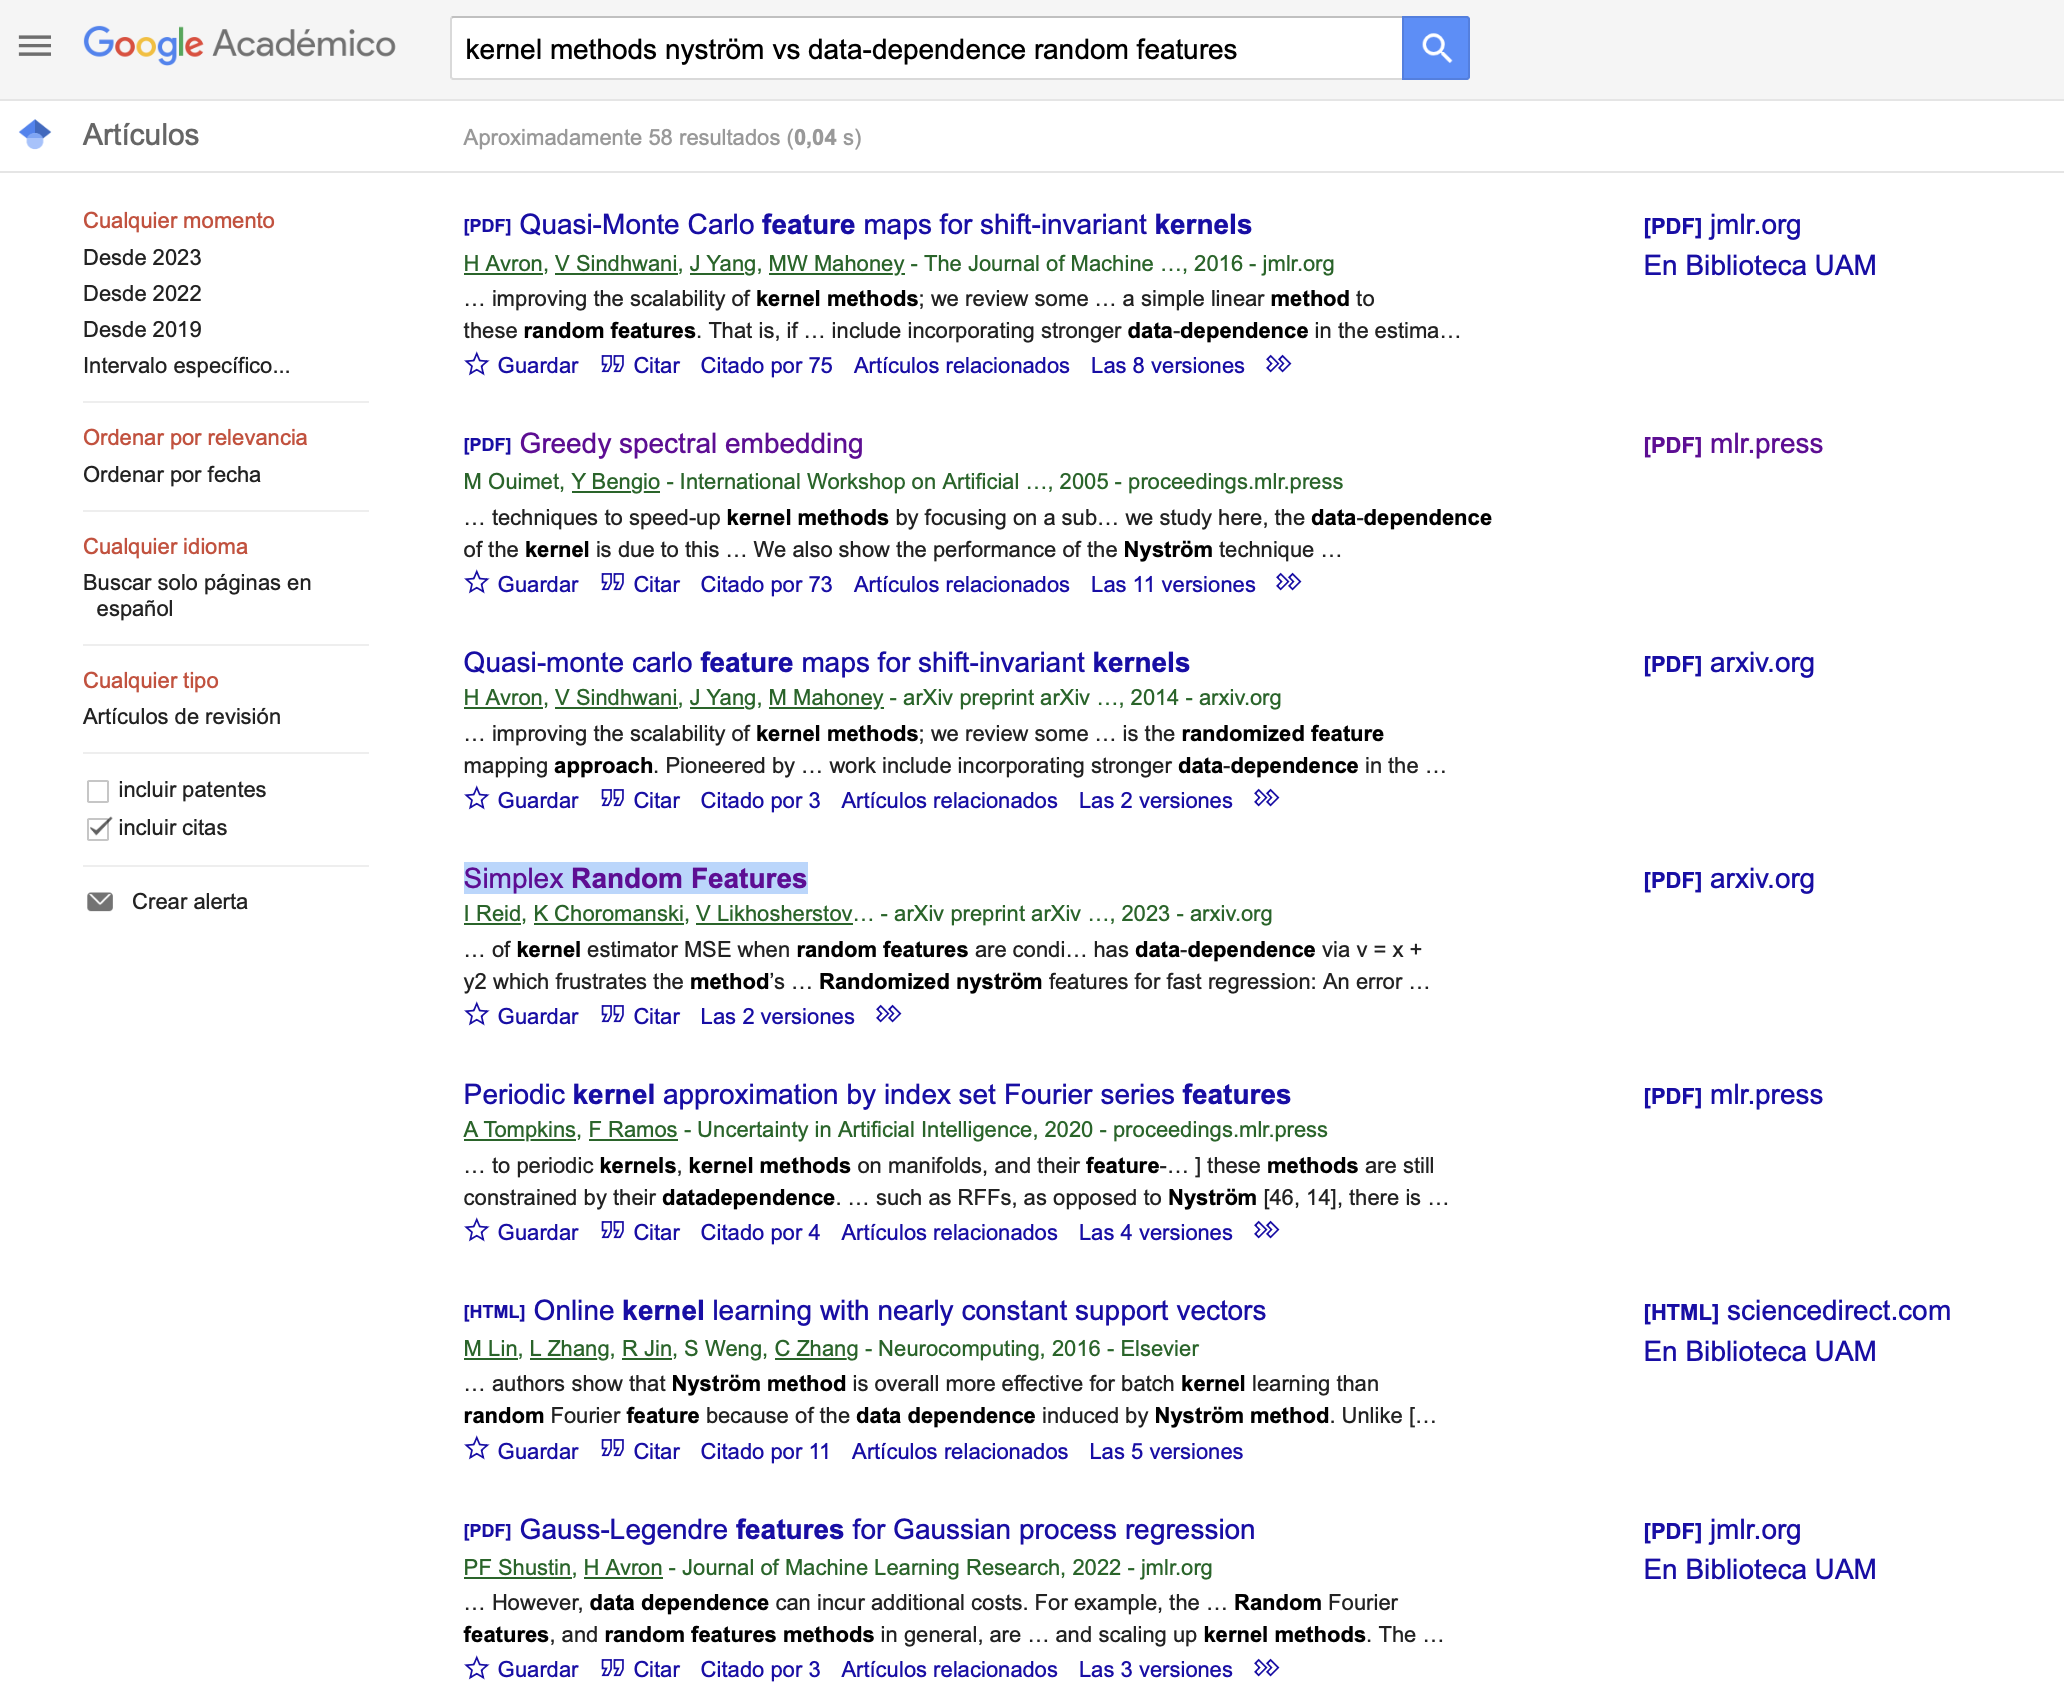
\includegraphics[height=0.7\textheight]{08_Random_features_for_kernel_approximation/google-schoolar.png}
  \centering
\end{figure}
  
\end{frame}

\begin{frame}
  \frametitle{Questions}
\begin{itemize}
  \item Why are there no comparisions articles? 
  \item The hypothesis was wrong?
  \item Why there are no comparative between algorithm and spectral sparsity. 
  \item How relevant is spectral sparsity?
  \item If it is important why not a lineal combination models and adjust the coefficient by some spectral approximation or heuristic?
\end{itemize}

\textbf{This survey would indirectly answer some of the questions }

\end{frame}

\begin{frame}
  \frametitle{Taxonomy}

  \begin{figure}[t]
    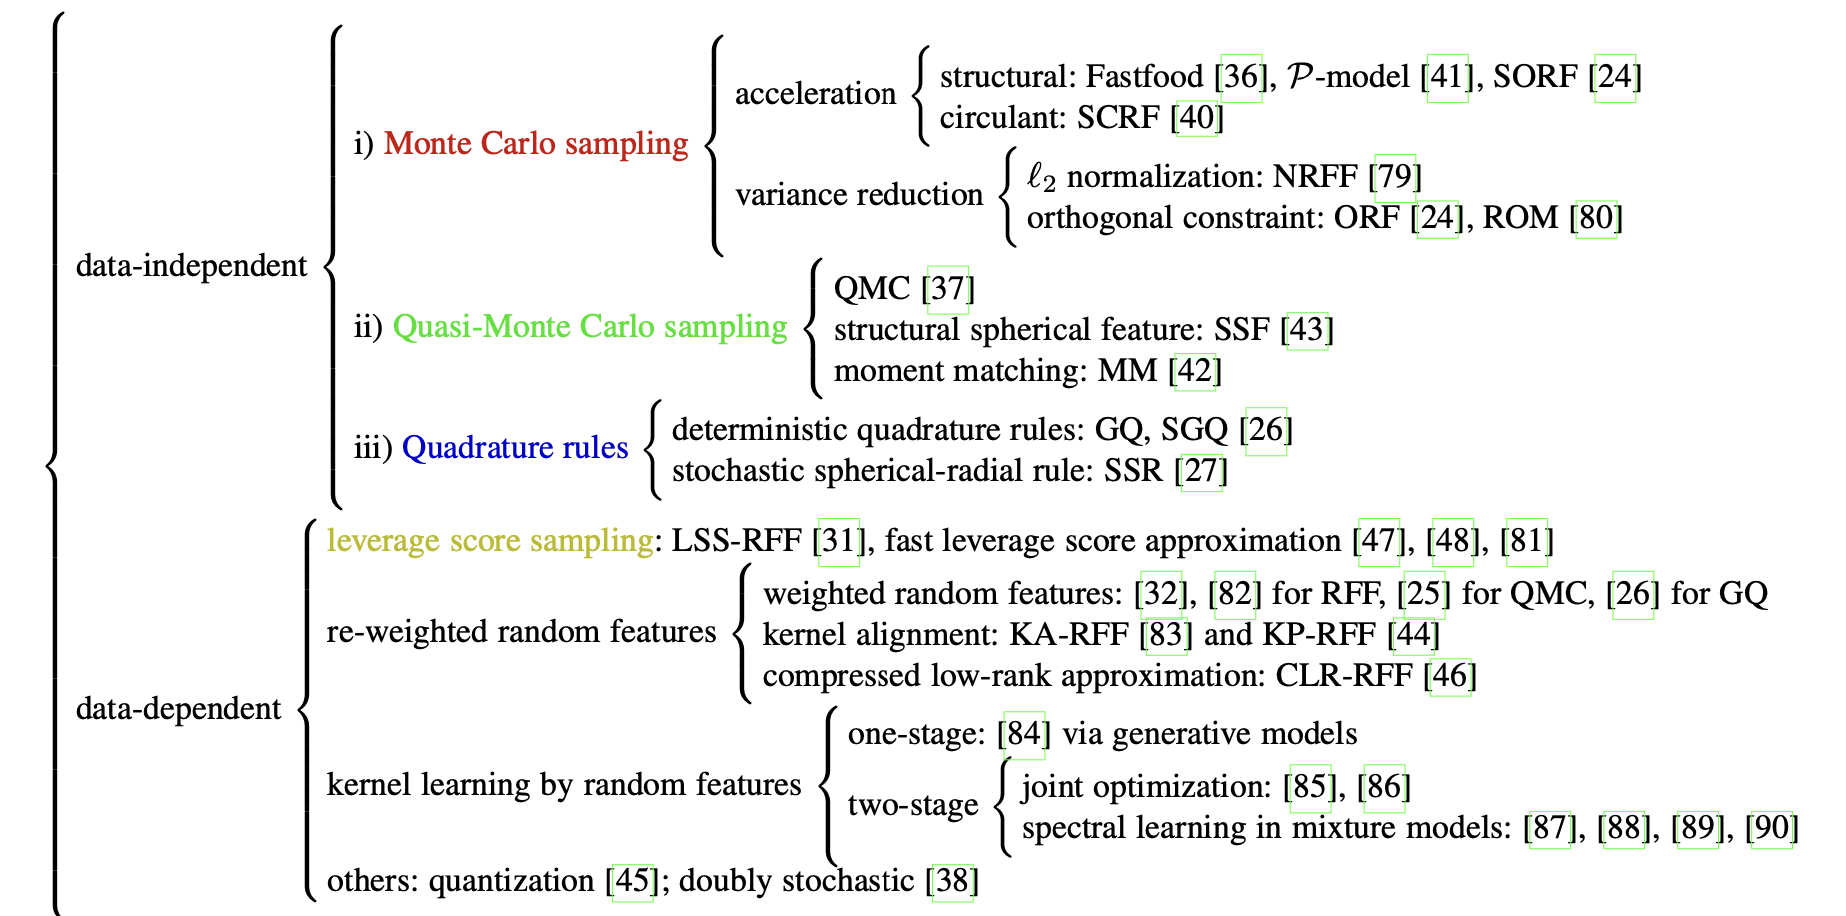
\includegraphics[height=0.8\textheight]{08_Random_features_for_kernel_approximation/taxonomy-of-representative-rf.png}
    \centering
  \end{figure}
\end{frame}

\begin{frame}
  \frametitle{Space and time complexities: No clear difference}
  \begin{figure}[t]
    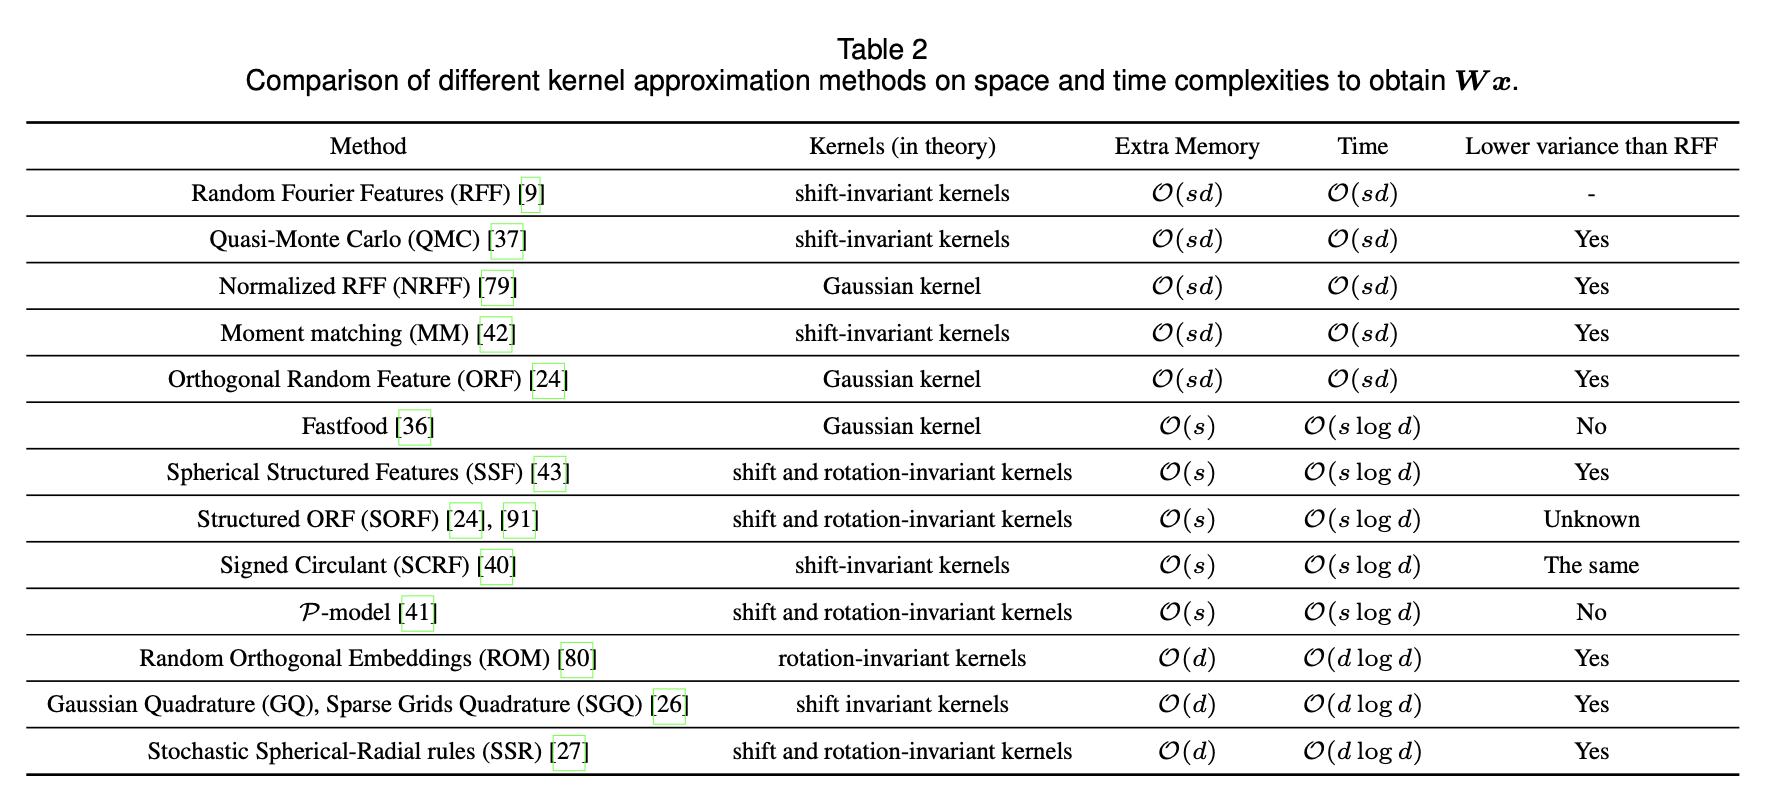
\includegraphics[height=0.8\textheight]{08_Random_features_for_kernel_approximation/comparasion-of-different-kernel-approximation-complexities.png}
    \centering
  \end{figure}
  
\end{frame}

\begin{frame}
  \frametitle{Models:}

  Here we test various random features based algorithms:
  
  \begin{center}
    \begin{tabular}{|c|c|}
    \hline
    Data-independient & Data-dependient \\
    \hline
    RFF & LS-RFF\\
    ORF & \\
    SORF & \\
    ROM & \\
    Fastfood & \\
    QMC & \\
    SSF & \\
    GQ & \\
    \hline
    \end{tabular}
    \end{center}
    
    

\textbf{Biased tests!}
\end{frame}

\begin{frame}
  \frametitle{Datesets: }

  \begin{figure}[t]
    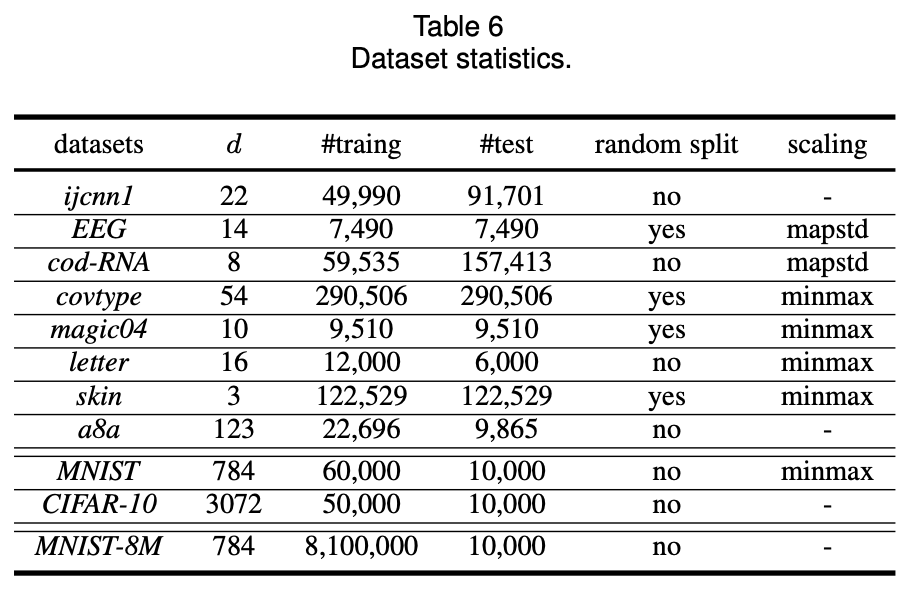
\includegraphics[height=0.8\textheight]{08_Random_features_for_kernel_approximation/datasets.png}
    \centering
  \end{figure}

\end{frame}
  

\begin{frame}
  \frametitle{Results:}

  \begin{figure}[t]
    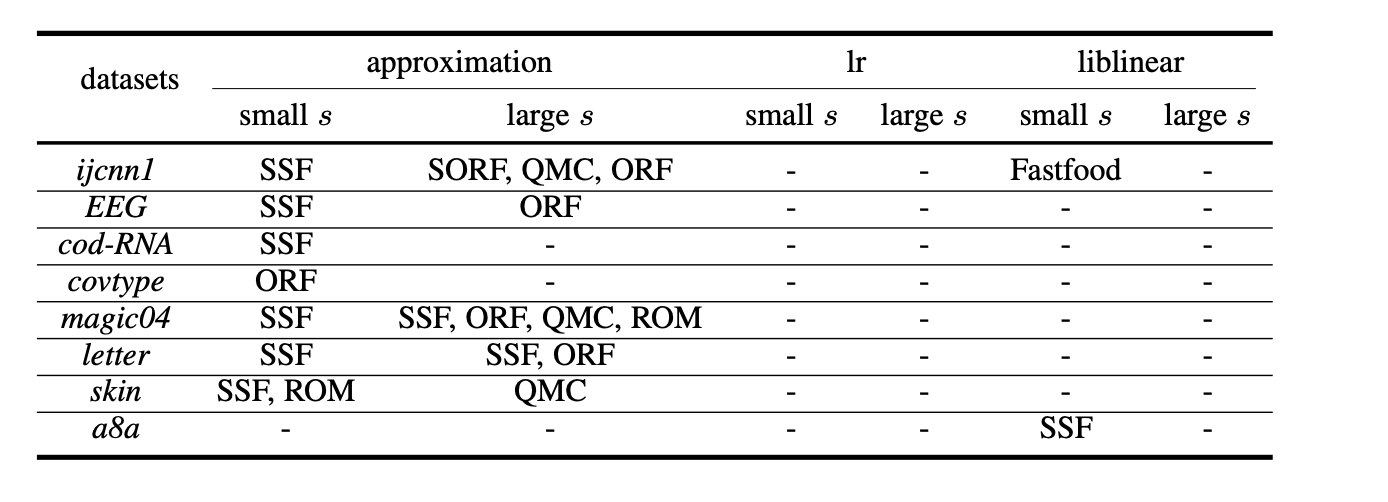
\includegraphics[width=\textwidth]{08_Random_features_for_kernel_approximation/results.png}
    \centering
  \end{figure}
  \begin{itemize}
    \item Approximation: small (SSF: 8/10), large (ORF 4/10, QMC: 3/10, SSF:  2/10). 
    \item Lineal regression: Adjusting the model kernel error are alleviated. 
  \end{itemize}
  

\end{frame}

\begin{frame}
  \frametitle{Having in mind taxonomy}

  \begin{itemize}
    \item SSF: data independent, Quasi-Monte Carlo sampling. 
    \item ORF: data independent, Monte Carlo sampling.  
    \item  QMC:  data independent, Quasi-Monte Carlo sampling.
  \end{itemize}

  \textbf{Where is LS-RFF?} (See appendix B)
  \begin{itemize}
    \item Highest (except ijcnn1) approximation error. 
    \item Most expensive time cost. 
  \end{itemize}

\end{frame}

\begin{frame}
  \frametitle{Why they did not test data indepence techniques? }
\begin{itemize}
  \item Not worthy? (A bit weird) 
\end{itemize}
  
\end{frame}


\begin{frame}
  \frametitle{Monte Carlo sampling based approaches }
% imgs/08_Random_features_for_kernel_approximation/montecarlo-sampling-based.jpeg
\begin{figure}[t]
  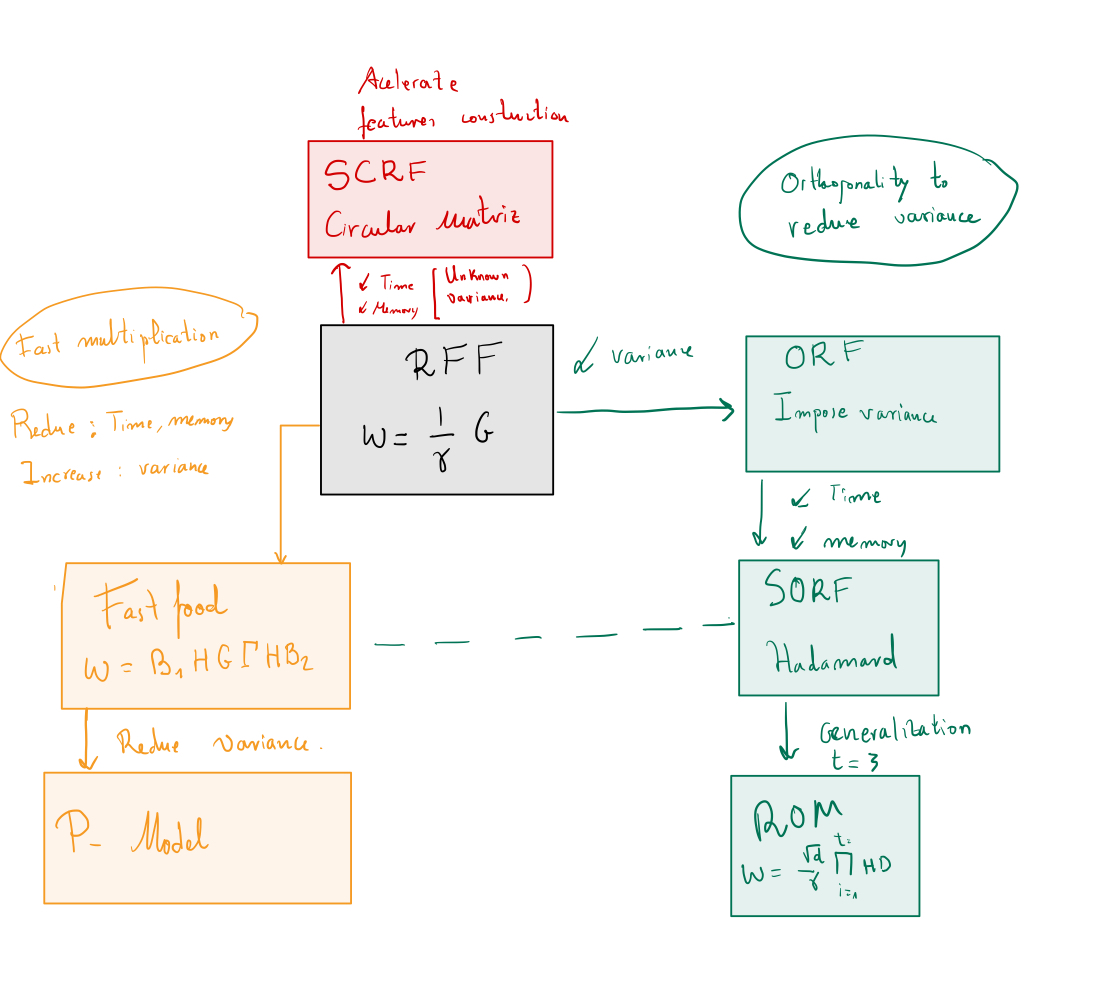
\includegraphics[height=0.95\textheight]{08_Random_features_for_kernel_approximation/montecarlo-sampling-based.jpeg}
  \centering
\end{figure}


\end{frame}


\begin{frame}
  \frametitle{Hadamard matrix (wikipedia)} 

  The Hadamard matrix can be constructed using the Sylvester construction, which involves recursively combining smaller Hadamard matrices to form larger ones.

Start with the $1 \times 1$ Hadamard matrix $H_1 = [1]$.
To construct the $2n \times 2n$ Hadamard matrix $H_{2n}$, form the matrix

  $$H_{2n} = \begin{bmatrix} H_n & H_n \\ H_n & -H_n \end{bmatrix}.$$

Using this construction, we can generate Hadamard matrices of any power of 2 size. For example, we can construct the $4 \times 4$ Hadamard matrix as follows:

$$H_4 = \begin{bmatrix} H_2 & H_2 \\ H_2 & -H_2 \end{bmatrix} = \begin{bmatrix} 1 & 1 & 1 & 1 \\ 1 & -1 & 1 & -1 \\ 1 & 1 & -1 & -1 \\ 1 & -1 & -1 & 1 \end{bmatrix}.$$

\end{frame}


\begin{frame}
  \frametitle{Walsh-Hadamard matrix }
  Rearrange the rows of the matrix according to the number of sign change of each row.
  

  $$
  W_4 = \frac{1}{\sqrt{4}} \begin{bmatrix}
  1 & 1 & 1 & 1 \\
  1 & 1 & -1 & -1 \\
  1 & -1 & -1 & 1 \\
  1 & -1 & 1 & -1 \\
  \end{bmatrix}
  $$
  
  Note that the Walsh matrix of size $4$ is equivalent to the second-order Hadamard matrix that I gave earlier.

\end{frame}


\begin{frame}
  \frametitle{Quasi-Monte Carlo Sampling}

  \textbf{Hypothesis:} $p$ factorizes with respect to the dimension
  \begin{equation*}
    p(x) = \prod_{j=1}^d p_j(x_j)
  \end{equation*}

  QMC transform the integral to 

  \begin{equation*}
    k(x - x')
    = 
    \int_{[0,1]^d}
    \exp(
      i(x-x')^T
      \phi^{-1}(t)
    ) dt,
  \end{equation*}
  where $\phi^{-1}(t) = (\phi_1^{-1}(t_1), \ldots, \phi_d^{-1}(t_d))$
  where $\{t\}$ is a low discrepancy sequence. 
  \begin{equation*}
    W = [\phi_1^{-1}(t_1), \ldots, \phi_d^{-1}(t_s)]
  \end{equation*}
\end{frame}


\begin{frame}
  \frametitle{SSF: Spherical structured feature maps for kernel approximation}
   It improves the space and time complexities of QMC for approximating shift- and rotation-invariant kernels

  SSF generates points  $$\{v_1, v_2, \ldots, v_s\}$$
    asymptotically uniformly distributed on the sphere 
    $S_{d-1}$and constructs the transformation matrix as 
  
  $$W_{\text{SSF}} = \left[\Phi^{-1}(t) v_1, \Phi^{-1}(t) v_2, \ldots, \Phi^{-1}(t) v_s \right]^T \in \mathbb{R}^{s \times d},$$
  where $\Phi^{-1}(t)$ is the inverse of the cumulative distribution function of the standard normal distribution evaluated at $t$.
\end{frame}

\begin{frame}
  \frametitle{}

  \begin{equation*}
    V =
    \frac{1}{\sqrt{d/s}}
    \begin{bmatrix}
      \Re F_\Lambda &  - \Im F_\Lambda \\
      \Im F_\Lambda & \Re F_\Lambda \\
    \end{bmatrix}
  \end{equation*}
  where  $F_\Lambda$  consiste of the row of the Fourier discrete matrix. 

  The discrete Fourier transform (DFT) matrix is defined as:

  $$
  F_{N}=\frac{1}{\sqrt{N}}\begin{pmatrix}
  1 & 1 & 1 & \cdots & 1 \\
  1 & w_{N} & w_{N}^{2} & \cdots & w_{N}^{N-1} \\
  1 & w_{N}^{2} & w_{N}^{4} & \cdots & w_{N}^{2(N-1)} \\
  \vdots & \vdots & \vdots & \ddots & \vdots \\
  1 & w_{N}^{N-1} & w_{N}^{2(N-1)} & \cdots & w_{N}^{(N-1)^{2}}
  \end{pmatrix},
  $$
  

  where $w_N = e^{-2\pi i/N}$ is a primitive $N$-th root of unity. 
  
\end{frame}

\begin{frame}
  The matrix $F_N$ is a unitary matrix and its inverse is given by the Hermitian transpose, i.e., $F_N^{-1} = F_N^H$.


$$ F = \frac{1}{2}
\begin{pmatrix}
1 & 1 & 1 & 1 \\
1 & i & -1 & -i \\
1 & -1 & 1 & -1 \\
1 & -i & -1 & i
\end{pmatrix}
$$

The selection of $d^2$ rows from $F$ is done by minimizing the discrete Riesz 0-energy such that the points spread as evenly as possible on the sphere.

\end{frame}

\section{Data dependent algorithm}

\subsection*{Leverage score based sampling}

\begin{frame}
  \frametitle{Leverage score based sampling: main idea}
Generate samples $w$ from a distribution $q$. 

Feature mapping: 
\begin{equation}
  \varphi_q(x)
  =
  \frac{1}{\sqrt{s}}
  \left(
    \sqrt{\frac{p(w_1)}{q(w_1)}} e^{-i w_1^T x},
    \ldots
    \sqrt{\frac{p(w_s)}{q(w_s)}} e^{-i w_s^T x}
  \right)^T
\end{equation}
  
\end{frame}

\begin{frame}
  \frametitle{How to design $q$}
  Let define ridge leverage function:
  \begin{equation}
    l_\lambda(w_i)
    =
    p(w_i)
    z_{p,w_i}^T(X)(K + n \lambda I)^{-1}
    z_{p,w_i}(X),
  \end{equation}
  where $\lambda$ s the KRR regularization parameter.

  Define
  \begin{equation}
    d_K^\lambda
    = 
    \int_{\R^d} l_\lambda(w) dw
    = 
    tr[K(K + n \lambda I)^{-1}].
  \end{equation}
  Number of effective degrees of freedom (independent parameters in a learning problem)
 $d^{\lambda} << n$

 {$q$ is designed as}
  \begin{equation}
    q(w)
    = 
    \frac{l_\lambda(w)}{d^\lambda_K}.
  \end{equation}

\end{frame}

\begin{frame}
  \frametitle{Improvements}
  \begin{itemize}
    \item Cost $K$ approximation and inverse ($O(n^3)$)
    \item LS-RFF uses a subset of data to approximate $K$. ($O(ns^2 + s^3)$).
    \item SLS-RFF (Surrogate Leverage Score-RFF) to avoid inverting an $s \times s$ matrix.$O(ns^2)$ same complexity as RFF.    
  \end{itemize}


\end{frame}

\begin{frame}
  \frametitle{Re-weighted random features}

  \begin{itemize}
    \item KA-RFF (Kernel Alignment-RFF) : It pre-computes a large
    number of random features that are generated by RFF, and then
    select a subset of them by solving a simple optimization problem
    based on kernel alignment. In particular, the optimization
    problem is

    \begin{equation}
      \max_{a \in P_J}
      \sum_{n}^{i,j = 1} y_i y_j
      \sum_{t = 1}^J a_t z_p(x_i, w_t)z_p(x_j, w_t).
    \end{equation}
    \item KP-RFF (Kernel Polarization-RFF) and CLR-RFF (Compression Low Rank-RFF): It first generates a
    large number of random features by RFF and then selects a subset
    from them using an energy-based scheme or solving and optimization problem.
  \end{itemize}

  
\end{frame}

\begin{frame}
  \frametitle{Hilbert coreset construction problem}

  The problem of building a small,
weighted subset of the data that approximates the full dataset,
is known as the \textbf{Hilbert coreset construction problem}.
Ans some solution: 
\begin{itemize}
  \item Greedy iterative geodesic ascent,
  \item Frank-Wolfe based methods, 
  \item Johnson-Lindenstrauss random projection. 
\end{itemize}

\end{frame}

\begin{frame}
  \frametitle{Kernel learning by random features}

  Construct random features using sophisticated learning techniques, e.g., by learning the spectral distribution
of kernel from the data.

\begin{itemize}
  \item Representative approaches in this class often involve a one-
  stage or two-stage process. 
  \begin{enumerate}
    \item Learns the random features,
    \item and then incorporates them into kernel methods for prediction.
  \end{enumerate}
  \item Example: leverage sampling and random features selection. 
  \item One-stage algorithms aim to simultaneously learn the spectral
  distribution of a kernel and the prediction model by solving a
  single joint optimization problem or using a spectral inference
  scheme. 
\end{itemize}

\end{frame}




\section{Computational cost}
\begin{frame}
  \frametitle{computational cost}
  Random Fourier Features  \cite{li2021sharp}:  reducing the computational complexity (roughly from $O(n^3)$ in time and $O(n^2)$ in space to $O(n^2)$ and $O(n \sqrt{n})$ respectively) without having to trade-off the statistical prediction accuracy.
  \begin{center}
    \resizebox{\textwidth}{!}{
    \begin{tabular}{ c | c |c |c | c}
     Step & Task & Theory & Cost  & Memory \\ 
     \hline
       % step
       1 
       % Task
      & Sampling Fourier components $u_1, \ldots u_m$ from $p(u)$.
      & % Theory 
        Inverse transform sampling, Accept or reject, Montecarlo. 
      & % cost 
      O(1)
      & % Memory 
      O(m)
      \\  
      % step------------
      2  
      & % Task
      Compute
      $
      z_f(x) = \left(
        \sin(u_1^T x), \cos(u_1^T x), 
        \ldots,
        \sin(u_m^T x), \cos(u_m^T x)
      \right)
      $
      % Theory 
      & 
      & % cost 
        O(m)
      & O(2m)
    \end{tabular}
    }
    \end{center}


    % nystrom
    Nyström
    \begin{center}
      \resizebox{\textwidth}{!}{
      \begin{tabular}{ c | c |c |c | c}
       Step & Task & Theory & Cost  & Memory \\ 
       \hline
         % step --------------
         1 
         % Task
        & Sampling
        & % Theory 
          
        & % cost 
        O(m)
        & % Memory 
        O(m)
        \\  
        % step------------
        2  
        & % Task
        constructing a low rank matrix by  
     $\hat{K}_r
      = 
      K_b 
      \hat{K}^\dagger 
      K_b^T.$
        % Theory 
        & 
        SVD and matrix multiplication
        & % cost 
        $O(n^3)$
        & $O(m^2)$
        \\
      \end{tabular}
      }
      \end{center}
      
      \begin{center}
        {
          \resizebox{\textheight}{!}{
        \begin{tabular}{ c |c | c}
          Training model & Cost  & Memory \\ 
         \hline
         Ridge regression 
         &
         $O(m^2(N+m))$
        & 
        $O(mn + n)$ 
        \\
        KRR
         &
         $O(n^3)$
        & 
        $O(n^2)$
        \\
        SVM
         &
         $O(n^2)$ or $O(n^3)$ 
        & 
        $O(n^2)$
        \\
        Backpropagation one layer
        &
        $O(n o d)$  (o output, d: mini batch size )
       & 
       $O(n o)$
        \end{tabular}
        }
        }
        \end{center}
  
\end{frame}
